\documentclass{beamer}
\usetheme{metropolis}
\usepackage{graphicx}
\usepackage{subcaption}
\usepackage{hyperref}
\usepackage{tcolorbox}
\title{Algebra-Based Physics-1: Mechanics (PHYS135A-01): You Have Learned A Lot}
\date{\today}
\author{Jordan Hanson}
\institute{Whittier College Department of Physics and Astronomy}

\begin{document}
\maketitle

\section{You Have Learned A Lot}

\begin{frame}{You Have Learned A Lot}
\scriptsize
\begin{enumerate}
\scriptsize
\item Unit 0: \textbf{Chapters - 18.1 - 18.5}, \textbf{Chapters 19.1 - 19.3}
\begin{itemize}
\scriptsize
\item Unit analysis, kinematics, and Newton's Laws
\item Work and energy, momentum
\item Electrostatics, I
\item The Coulomb Force, and Newton's Second Law for electric charges
\item The concept of an electric field
\item Electrostatics, II
\item Potential energy and charge, voltage
\item Potential energy and fields, point charges
\item Electrostatics in biology
\end{itemize}
\scriptsize
\item Unit 1: \textbf{Chapters 19.4 - 19.7}, \textbf{Chapters 20.1 - 20.5, 20.7}
\begin{itemize}
\scriptsize
\item Capacitors and capacitance
\item Equipotential lines, capacitance, and capacitors
\item Capacitors in series and in parallel, energy considerations
\item Current and DC circuits
\item DC current and resistance, Ohm's law
\item Energy and power in DC current
\item AC current and waveforms
\end{itemize}
\end{enumerate}
\end{frame}

\begin{frame}{You Have Learned A Lot}
\scriptsize
\begin{enumerate}
\scriptsize
\item Unit 2: \textbf{Chapters 21.1 - 21.4, 21.6}
\begin{itemize}
\scriptsize
\item DC circuit basics
\item Resistors in series and parallel, electromotive force (EMF)
\item Kirchhoff's rules
\item Voltmeters and ammeters
\item RC circuits
\end{itemize}
\scriptsize
\item Unit 3: \textbf{Chapters 22.1 - 22.4}, \textbf{Chapters 22.7 - 22.9}
\begin{itemize}
\scriptsize
\item Magnetostatics I
\item Magnets, ferromagnetic and electromagnetic
\item Magnetic fields and field lines, force on moving charge
\item Magnetic applications I: mass spectrometry
\item Magnetostatics II
\item Force on current carrying conductor, torque on current loop
\item Amp\`{e}re's Law: magnetic fields created by current
\item Magnetic applications II: fusion reactors
\end{itemize}
\end{enumerate}
\end{frame}

\begin{frame}{You Have Learned A Lot}
\scriptsize
\begin{enumerate}
\scriptsize
\item Unit 4: \textbf{Chapters 23.1 - 23.5, 23.7, 23.9}, \textbf{Chapters 23.9 - 23.12}
\begin{itemize}
\scriptsize
\item Magnetic induction
\item Induced EMF, magnetic flux
\item Faraday's Law
\item Motional EMF, generators, transformers
\item AC circuits
\item Inductors
\item RL circuits
\item RLC circuits
\end{itemize}
\scriptsize
\item Unit 5: \textbf{Chapters 24.1 - 24.4}, \textbf{Chapters 25.1 - 25.3, 25.6}, \textbf{32.1 - 32.4}
\begin{itemize}
\scriptsize
\item Electromagnetic waves
\item Maxwell's Equations
\item Electromagnetic wave production
\item Electromagnetic spectrum and energy
\item Geometric optics: ray-tracing, reflection, refraction, lenses
\item Nuclear physics in medicine
\item Diagnostics and medical imaging
\item Biological effects of ionizing radiation
\end{itemize}
\end{enumerate}
\end{frame}

\begin{frame}{You Have Learned A Lot}
\scriptsize
\begin{itemize}
\item $\vec{v}_{\rm ave} = \Delta\vec{x}/\Delta t$ ... Definition of average velocity involving vectors.
\item $x(t) = \frac{1}{2}at^2 + v_{\rm i} t + x_{\rm i}$ ... One-dimensional displacement with constant acceleration.
\item $v(t) = v_{\rm i} + a t$ ... One-dimensional velocity with constant acceleration. 
\item $\vec{F}_{\rm net} = m\vec{a}$ ... Newton's 2nd Law.
\item $W = \vec{F} \cdot \vec{x}$ ... Definition of work involving vectors.
\item $W = Fx\cos\theta$ ... Definition of work, with $\theta$ as angle between force and displacement.
\item $KE = \frac{1}{2} m v^2$ ... Kinetic energy.
\item $W = \Delta KE = KE_{\rm f} - KE_{\rm i}$ ... Work energy theorem.
\item $KE_{\rm i} + PE_{\rm i} = KE_{\rm f} + PE_{\rm f}$ ... Energy conservation.
\item $\vec{p} = m\vec{v}$ ... Definition of momentum involving vectors.
\item $\vec{p}_{\rm tot,i} = \vec{p}_{\rm tot,f}$ ... Conservation of momentum.
\item $\tau = I\alpha$ ... Netwon's 2nd Law for rotating objects, with torque, moment of inertia, and angular acceleration.
\item $KE_{\rm rot} = \frac{1}{2}I \omega^2$ ... Rotational kinetic energy.
\item $L = I \omega$ ... Angular momentum.
\end{itemize}
\end{frame}

\begin{frame}{You Have Learned A Lot}
\scriptsize
\begin{itemize}
\item $\vec{a} = a_x \hat{i} + a_y \hat{j}$ ... Component notation for 2D vector
\item $\vec{a} + \vec{b} = (a_x + b_x)\hat{i} + (a_y + b_y)\hat{j}$ ... Adding vectors
\item $\vec{a} - \vec{b} = (a_x - b_x)\hat{i} + (a_y - b_y)\hat{j}$ ... Subtracting vectors
\item $|\vec{a}| = \sqrt{a_x^2 + a_y^2}$ .. Magnitude of a 2D vector
\item $a_x = |\vec{a}|\cos\theta$ ... x-component of a 2D vector
\item $a_y = |\vec{a}|\sin\theta$ ... y-component of a 2D vector
\item $\vec{a} \cdot \vec{b} = a_x b_x + a_y b_y$ ... Dot product of two vectors
\end{itemize}
\begin{itemize}
\item $\vec{E} = \frac{k Q}{r^2} \hat{r}$ ... Coulomb field of a charge $Q$.
\item $k = 8.99 \times 10^{9}$ N C$^{-2}$ m$^{2}$ ... Constant of proportionality for Coulomb field.
\item $\vec{F} = q \vec{E}$ ... Force on a charge $q$ in the presence of an $\vec{E}$-field.
\item $\vec{F} = m\vec{a}$ ... Newton's 2nd Law.
\item $m = \rho V = \frac{4}{3}\pi r^3 \rho$ ... Mass of a sphere with volume $V$, density $\rho$, and radius $r$.
\item $PE = q V$ ... Relationship between potential energy, charge, and voltage.
\item $V_{AB} = Ed$ ... Relationship between voltage between points A and B, a distance $d$ apart, for a constant E-field $E$.
\end{itemize}
\end{frame}

\begin{frame}{You Have Learned A Lot}
\scriptsize
\begin{itemize}
\item $Q = CV$ ... Relationship between capacitance, charge, and voltage.
\item $C_{tot} = C_1 + C_2 + C_3 + ...$ ... Capacitors in parallel.
\item $C = A\epsilon_0/d$ ... Capacitance of a parallel-plate capacitor.
\item $\epsilon_0 = 8.85 \times 10^{-12}$ F/m
\item $C_{tot}^{-1} = C_1^{-1} + C_2^{-1}$ ... Total capacitance of two capacitors in series.
\item $I = \Delta Q/\Delta t$ ... Definition of current.
\item $\Delta V = I R$ ... Ohm's Law, relating resistance $R$, current $I$, and voltage $\Delta V$.
\item $U = \frac{1}{2} C V^2$ ... Energy stored in a capacitor.
\item $P = U/T$ ... Power consumed in a system, assuming $U$ is energy or work done, and $T$ is time duration.
\item $y(x) = mx + b$ ... Linear function with slope $m$, and y-intercept $b$
\item $m = \Delta y / \Delta x$ ... Formula for slope.
\item $V = i R$ ... Ohm's Law, with $V$ for voltage, $i$ for current, and $R$ for resistance.
\item $R_{\rm tot} = R_1 + R_2 + ...$ ... Resistors in \textit{series.}
\item $R_{tot}^{-1} = R_1^{-1} + R_2^{-1}$ ... Total resistance of two resistors in parallel.
\item $P = IV$ ... The power consumed by a device that draws a current $I$ at a voltage $V$.
\end{itemize}
\end{frame}

\begin{frame}{You Have Learned A Lot}
\scriptsize
\begin{itemize}
\item $(x \pm \sigma_x) + (y \pm \sigma_y) = (x+y) + \sqrt{\sigma_x^2 + \sigma_y^2}$ ... Adding two averages with errors.
\item $\hat{i} \times \hat{j} = \hat{k}$, $\hat{j} \times \hat{k} = \hat{i}$, $\hat{k} \times \hat{i} = \hat{j}$ ... The direction of the \textit{cross-product} follows this pattern.  Reversing the order of any two vectors introduces a minus sign.
\item $\hat{i} \times \hat{i} = 0$, $\hat{j} \times \hat{j} = 0$, $\hat{k} \times \hat{k} = 0$ ... The \textit{cross-product} is zero when both vectors are parallel.
\item $|\vec{a} \times \vec{b}| = |\vec{a}||\vec{b}|\sin\theta$ ... The magnitude of the cross-product of two vectors $\vec{a}$ and $\vec{b}$, given the angle $\theta$ between them.
\item $\vec{F} = i\vec{L} \times \vec{B}$ ... The Lorentz force, by a magnetic field $\vec{B}$ on a \textit{current} $i$ of length and direction $\vec{L}$.
\item $\vec{F} = q\vec{v} \times \vec{B}$ ... The Lorentz force, one version.
\item $\vec{F} = i\vec{L} \times \vec{B}$ ... The Lorentz force, another version.
\item $\vec{\tau} = \vec{r} \times \vec{F}$ ... Definition of torque.
\item $\vec{\tau} = \vec{\mu} \times \vec{B}$ ... Torque on a current carrying loop in a uniform B-field.
\item $\vec{\mu} = Ni\vec{A}$ ... Definition of the magnetic moment.
\item $B = (\mu_0 I)/(2\pi r)$ ... The magnetic field $B$ \textit{caused} by the current $I$ a distance $r$ away.
\end{itemize}
\end{frame}

\begin{frame}{You Have Learned A Lot}
\scriptsize
\begin{itemize}
\item $\epsilon = -N \Delta \phi_m /\Delta t$ ... Faraday's Law
\item $\phi_m = \vec{B} \cdot \vec{A}$ ... Definition of magnetic flux
\item $\epsilon = -N \Delta \phi_m /\Delta t$ ... Faraday's Law
\item $\phi_m = \vec{B} \cdot \vec{A} = BA \cos(\theta)$ ... Definition of magnetic flux
\item $\epsilon(t) = \epsilon_0 \sin(\omega t)$ ... AC voltage generated by generator.  $\epsilon_0$ is proportional to $\omega$.
\item $P_{max} = V_{max}^2/R$ ... Max power of an AC generator.
\item $P_{ave} = \frac{1}{2} P_{max}$ ... Average power of an AC generator.
\item $\epsilon(t) = V_{max} \sin(\omega t)$ ... AC voltage signal.
\item $\omega = 2\pi f$ ... Angular frequency vs. frequency.
\item $\epsilon = -L \Delta I/\Delta t$ ... Faraday's Law, with inductance $L$
\item $\epsilon_2/\epsilon_1 = N_2/N_1$ ... Transformer equation
\item $\epsilon(t) = \epsilon_0 (2 \pi f) \cos(2\pi ft)$ ... Variation of induced voltage as a function of time
\item $v(t) = v_0 \sin(2\pi ft - \phi)$ ... Standard AC waveform, with amplitude $v_0$, in volts, frequency $f$, in Hertz, time $t$, in seconds, and phase $\phi$, in radians.
\item $X_{\rm C} = 1/(2\pi f C)$ ... The reactance of a capacitor with capacitance $C$, at frequency $f$.
\item $X_{\rm L} = 2\pi f L$ ... The reactance of an inductor with inductance $L$, at frequency $f$.
\item $Z_{\rm tot} = \sqrt{R^2 + (X_{\rm L} - X_{\rm C})^2}$ ... The total impedance of a series circuit with resistance $R$, and reactances $X_{\rm C}$ and $X_{\rm L}$.
\item $\tau = RC$ ... The time constant of an RC circuit.
\item $f_0 = \frac{1}{2\pi\sqrt{LC}}$ ... The resonance frequency of an RLC circuit.
\end{itemize}
\end{frame}

\begin{frame}{You Have Learned A Lot}
\scriptsize
\begin{itemize}
\item $c = f\lambda$ ... The relationship between speed of light, $c$, the frequency, $f$, and the wavelength, $\lambda$.
\item $c = 299,792,458$ m s$^{-1}$, or $c \approx 0.3$ m ns$^{-1}$.
\item $\bar{S} = E^2/(2c\mu_0)$ ... Average \textbf{intensity}, or W m$^{-2}$, of electromagnetic energy.
\item $c/n = f \lambda$ ... Relationship between the speed of light, $c$, the index of refraction, $n$, the frequency of an electromagnetic wave, $f$, and its wavelength, $\lambda$.
\item $c = 3.0 \times 10^8$ m s$^{-1}$ ... The speed of light in a vacuum, within 1 percent error.
\item $\sin(x)\cos(y) = \frac{1}{2}\left(\sin(x+y) + \sin(x-y)\right)$ ... Trigonometric identity.
\item $\Delta x = v \Delta t$ ... The relationship between displacement, constant velocity, and time duration.
\item \textbf{Optics:} Snell's Law states that, for an interface between two media with \textit{indices of refraction} $n_1$ and $n_2$, light leaves one medium with an angle $\theta_1$ and enters the second medium with an angle $\theta_2$ as follows:
\begin{equation}
n_1 \sin\theta_1 = n_2\sin\theta_2
\end{equation}
\noindent The two angles are defined with respect to vertical.
\item \textbf{Optics:} Fresnel's equations give the fraction of power (in light) that is reflected ($R$) or transmitted ($T$) by an interface between media with indices of refraction $n_1$ and $n_2$:
\begin{equation}
R = \left| \frac{n_1 - n_2}{n_1 + n_2} \right|^2 \label{eq:2}
\end{equation}
\end{itemize}
\end{frame}

\section{Think About it Another Way}

\begin{frame}{Think About it Another Way}
\begin{figure}
\centering
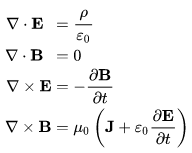
\includegraphics[width=0.3\textwidth]{max.png}
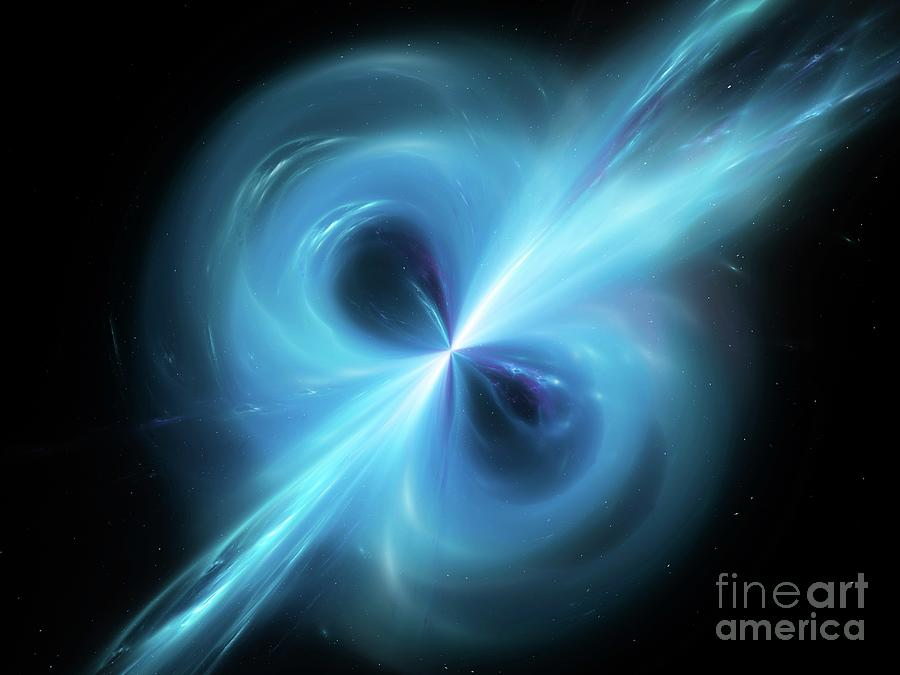
\includegraphics[width=0.25\textwidth]{field1.jpg}
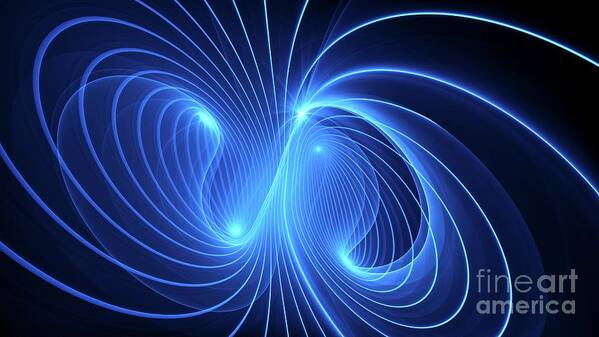
\includegraphics[width=0.35\textwidth]{field2.jpg}
\caption{\label{fig:1} All of the knowledge we have covered this semester can be derived from Maxwell's Equations, and the conservation of charge and energy.}
\end{figure}
\textbf{Is the Universe really like that?} ... I sure hope so.
\end{frame}

\section{Thank You}

\begin{frame}{Think About it Another Way}
\begin{figure}
\centering
\includegraphics[width=0.9\textwidth]{kids.jpg}
\caption{\label{fig:2} We are greatful to be able to share this endeavor with you.}
\end{figure}
\end{frame}

\end{document}
